\documentclass[runningheads]{llncs}

% General
% -------
\usepackage[labelfont={small,bf},textfont={small,it},skip=1pt]{caption}
\usepackage{graphicx}
\usepackage{booktabs}
\usepackage{caption}
\usepackage{tabularx}
\usepackage{subfigure}
\usepackage[normalem]{ulem}
\usepackage{fancyref}
\usepackage{xcolor}
\usepackage{float}
\usepackage{cite}
\usepackage{amssymb}
\usepackage[skip=0.1cm]{parskip}

\setlength{\textfloatsep}{0pt}
%\titlespacing*{\section}{0pt}{1.1\baselineskip}

\useunder{\uline}{\ul}{}

\newcommand{\eg}{{\it e.g.}}
\newcommand{\ie}{{\it i.e.}}
\newcommand{\etal}{{\it et al.}}
\newcommand{\AH}[1]{\textcolor{purple}{[AH: #1]}}
\newcommand{\xxx}[1]{\textcolor{red}{[#1]}}


\pagestyle{plain}

%%%%%%%%%%%%%%%%%%%%  TITLE/AUTHORS  %%%%%%%%%%%%%%%%%%%%%

\begin{document}

\title{Measuring the Availability and Response Times of Public Encrypted DNS Resolvers}
\author{}
\institute{}

%%%%%%%%%%%%%%%%%%%%  START OF DOCUMENT  %%%%%%%%%%%%%%%%%

\maketitle

\begin{sloppypar}
\abstract{
The Domain Name System (DNS) translates domains that are readable by humans to respective IP addresses. 
DNS traffic is traditionally unencrypted, which allows users' private information to be leaked. 
In response to these privacy risks, protocols for encrypting DNS have recently been deployed including DNS over HTTPS (DoH) and DNS over TLS (DoT).
Even with DoH, an individual's Internet traffic is not entirely hidden. 
The designated encrypted DNS server can still see and log those query requests. 
If most people rely on the same mainstream encrypted DNS providers, those providers will have access to incredibly large amounts of data and user information, which simply shifts the original privacy concerns from Internet Service Providers (ISPs) to mainstream encrypted DNS resolvers. 

In this paper we explore the reliability of encrypted DNS resolvers by measuring query response times from different global vantage points. 
We find that although most lesser-known resolvers have higher response times than well-known resolvers, which was expected, a selective group of non-mainstream resolvers operate better than mainstream resolvers. 
This allows users to expand their options of trusted recursive resolvers beyond those that are well-known. 
We present the sufficient options that users have for good performance while maintaining privacy.

\section{Introduction}\label{sec:intro}

The Domain Name System (DNS) is a critical component of the Internet's
infrastructure that translates human-readable domain names (\eg,
\texttt{google.com}) into Internet Protocol (IP) addresses~\cite{rfc1035}.
Most Internet communications begin with a client device sending DNS queries to
a recursive resolver, which in turn queries one or more name servers, which
ultimately refer the client to a server who can map the domain to an IP
address.
The \emph{response times} of these queries---the time 
to contact a recursive resolver, query various name servers, and return
the results---is important because the DNS underlies virtually all
communication on the Internet.  For example, loading a
web page, a browser must first resolve the domain names for each object on the
page before the objects themselves can be retrieved and rendered.  Thus, the
performance of DNS lookup is of utmost importance to application performance
such as web performance, as slow DNS lookup times will lead to slow web page
loads.

DNS did not originally take privacy and security into account: DNS queries
have historically been unencrypted, leaving users susceptible to
eavesdropping~\cite{dns-eavesdrop}; queries can also be intercepted and
manipulated to re-direct users to malicious websites~\cite{dns-redirect}.  To
address these types of privacy and security vulnerabilities, encrypted DNS
protocols have been developed and deployed, including DNS-over-HTTPS
(DoH)~\cite{rfc8484}, which is now deployed---and even enabled by default---in
many browsers.  DoH enables clients to communicate with recursive resolvers
over HTTPS, providing privacy and security guarantees that DNS previously
lacked.

For better or worse, most contemporary deployments of DoH have occurred in
browsers that provide limited options of
resolvers~\cite{ffChoices,chromeResolvers}.  If users continue to adopt
encrypted DNS and rely on a small set of recursive resolvers, these resolvers
will have increased visibility into data that was previously available to a
multitude of resolvers.  Such data includes queries that correspond to users'
web browsing histories.

\begin{table}[t]
    \centering
    \begin{tabular}{l|cccccc}
    \hline
    Browser & Cloudflare & Google & Quad9 & NextDNS & CleanBrowsing & OpenDNS
    \\
    \midrule
    Chrome    & \checkmark & \checkmark & & \checkmark & \checkmark & \checkmark \\
    Firefox  & \checkmark & & & \checkmark & & \\ 
    Edge   & \checkmark & \checkmark & \checkmark & \checkmark & \checkmark & \checkmark \\
    Opera            & \checkmark & \checkmark & & & & \\
    Brave            & \checkmark & \checkmark & \checkmark & \checkmark & \checkmark & \checkmark \\
    \bottomrule
    \end{tabular}
    \caption{Modern browsers provide only a few choices for encrypted DNS
    resolver, which we define as {\bf mainstream} resolvers.}
    \label{tab:SupportedResolvers}
\end{table}

\Fref{tab:SupportedResolvers} shows the DoH resolvers that have been deployed
to users of major browsers as of October 20,
2021~\cite{bravebrowser,edgebrowser,ffbrowser,chromebrowser,operabrowser}.  We
define the resolvers listed in~\Fref{tab:SupportedResolvers} as {\em
mainstream}.
Yet, many other DoH resolvers have been deployed that are currently
not in use by major browser deployments~\cite{dnscrypt}---in other words,
there are many non-mainstream DoH resolver deployments.  

Although DoH
addresses passive eavesdropping of DNS queries, it does not prevent resolvers
\emph{themselves} from seeing the contents of DNS queries.  Thus, some have
argued that major browser-based DoH deployments shift privacy concerns from
eavesdroppers to potential misuse by major DNS providers~\cite{vixie}.

Various previous studies have measured encrypted DNS performance, but they have mostly focused on mainstream DNS resolvers~\cite{borgolte2019dns,hounsel2020comparing,KResolver,lu2019end-to-end}.
In this paper, we expand on these previous studies, exploring the performance
of all encrypted DNS resolvers---from a variety of global (particularly
non-US) vantage points, as opposed to simply characterizing the mainstream DoH
providers from well-connected vantage points.
Towards this goal, we make the following contributions:
\begin{enumerate}
    \itemsep=-1pt
    \item We measure DoH response times a large list of resolvers, including
        both mainstream DoH resolvers that are included in major browser
        vendors {\em and} a large collection of non-mainstream resolvers.
%    \item We study whether users must use a major provider to experience acceptable DoH response times.
    \item We study how the performance of various DoH resolvers differ based
        on vantage point.
\end{enumerate}
\noindent
To our knowledge, this paper presents the first study of DoH performance
measurements for non-mainstream resolvers, as well as the first comparison of
DoH performance across a variety of vantage points, for a large number of
resolvers.
To perform these experiments, we developed and released an open-source
tool for measuring encrypted DNS performance to replicate and extend these
results, and to support further research on DoH performance.

The rest of the paper is organized as follows.  Section~\ref{sec:background}
provides background on DNS, including the origin of encrypted DNS and related
standards, and discusses related work.  Section~\ref{sec:method} details our research questions, the
experiments we conducted to study these questions, and the limitations of the
study.  Section~\ref{sec:results} presents the results of these experiments.
Section~\ref{sec:conclusion} concludes with a discussion of the implications
of these results and possible directions for future work. 


\section{Background}\label{sec:back}
The Domain Name System (DNS) translates human-readable domain names into Internet Protocol (IP) addresses, which are used to route traffic~\cite{dns-rfcs}.
These queries are traditionally unencrypted, which enables on-path eavesdroppers to intercept queries and manipulate responses.

Protocols for encrypting DNS traffic have been proposed, standardized, and deployed in recent years, including DNS-over-HTTPS (DoH) and DNS-over-TLS (DoT).
DoT was proposed by Hu et al. in 2016 to address the eavesdropping and tampering of DNS queries~\cite{8}.
It utilizes a dedicated port (853) to communicate with resolvers over a TLS connection.
In contrast, DoH--proposed by Hoffman et al. in 2018--establishes HTTPS sessions with resolvers over port 443~\cite{7}.
This design decision enables DoH traffic to blend in with traditional HTTPS traffic, making it difficult for network operators and eavesdroppers to intercept DNS queries and responses.
In short, DoH is designed to function in environments where DoT is more easily blocked.

However, encryption does not mean that DNS traffic is entirely invisible.
By design, recursive resolvers receive queries from clients and may perform additional queries to other name servers to resolve domain names.
In order for these resolvers to determine what additional queries they need to perform (or determine if the query can be answered from a cache), they must decrypt the queries that they receive from clients.
Thus, although DoT and DoH make it difficult for network operators and eavesdroppers to intercept DNS traffic, recursive resolvers \emph{themselves} are still able to log the queries that they receive from clients.

Most major browsers currently support DoH, including Brave, Chrome, Edge, Firefox, Opera, Safari, and Vivaldi.
Operating systems have also announced plans to implement DoH, including iOS, MacOS, and Windows~\cite{16,17,18,19,20,21,22}.
For this study, we chose to focus on DoH because it is more widely implemented than DoT.
Each of the aforementioned browsers and operating systems either currently support or have announced support for DoH, but not DoT~\cite{lack-of-dot-support}.

In this paper, we measure query response times and reachability for a large list of DoH resolvers, many of which are not available as default options in major browsers.
Previous studies measuring DoT and DoH response times largely focus on and compare the protocols as a whole, rather than the performance of individual resolvers~\cite{14}.
Our research specifically focuses on collecting measurements of the larger DoH ecosystem to better understand what options are practically available to DoH clients.


\section{Method}\label{sec:method}

In this section, we describe the metrics used and these metrics are measured with our experiment setup.

\subsection{Metrics}
To understand how non-mainstream resolvers function in relation to mainstream resolvers, we measure DNS query response times and ping times. 
DNS query response times were gathered using a custom tool, and ping times were gathered with MaxMind's GeoLite2 databases.

- Explain DNS query response times
- Explain ping times (latency)

\subsection{Experiment Setup}

\subsection{Limitations}
	- Measurements performed on a Debian operating system 
	- We don't measue page load times 
	
\section{Results}\label{sec:results}
In this section, we describe the results of our experiment. 

\begin{figure}[t!]
\centering
\subfigure[North America.]{%
\label{fig:Ohio_NA}%
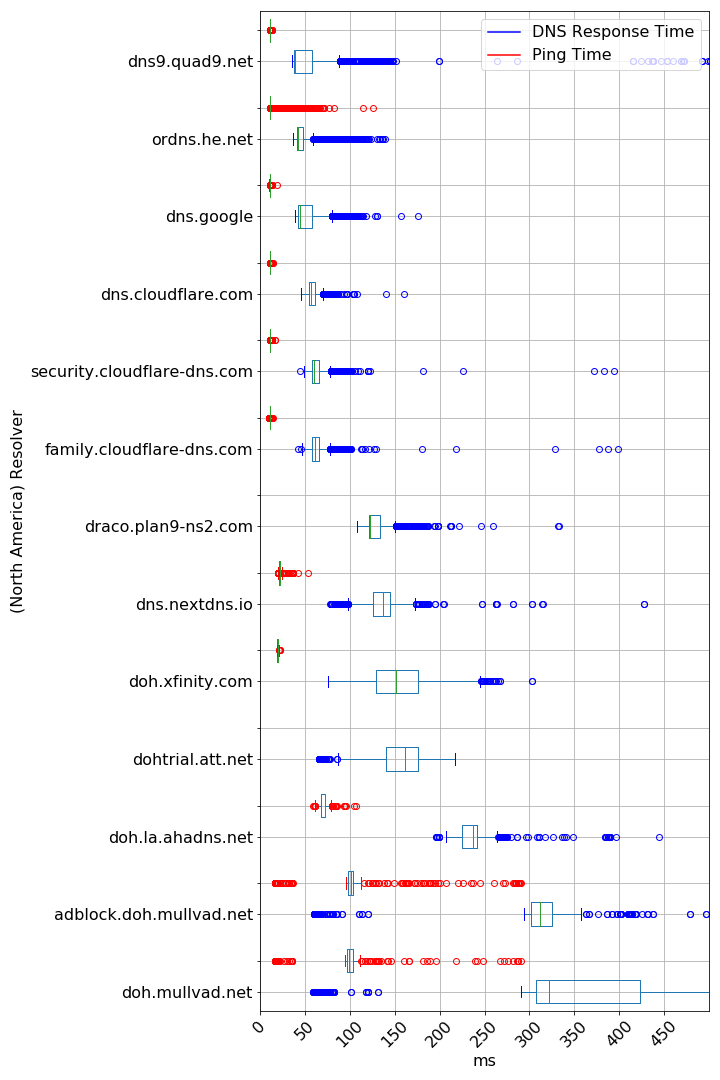
\includegraphics[height=2in]{figures/Ohio_North_America.png}}%
\hspace{8pt}%
\subfigure[Asia.]{%
\label{fig:Ohio_Asia}%
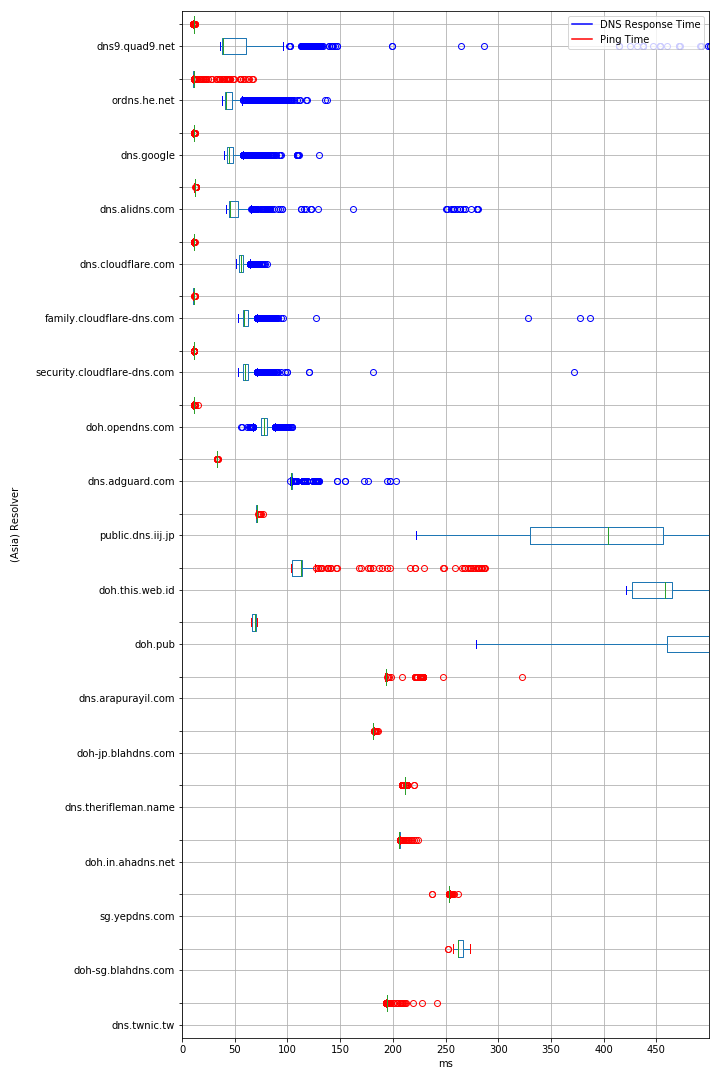
\includegraphics[height=2in]{figures/Ohio_Asia.png}}%
\hspace{8pt}%
\subfigure[Europe.]{%
\label{fig:Ohio_Europe}%
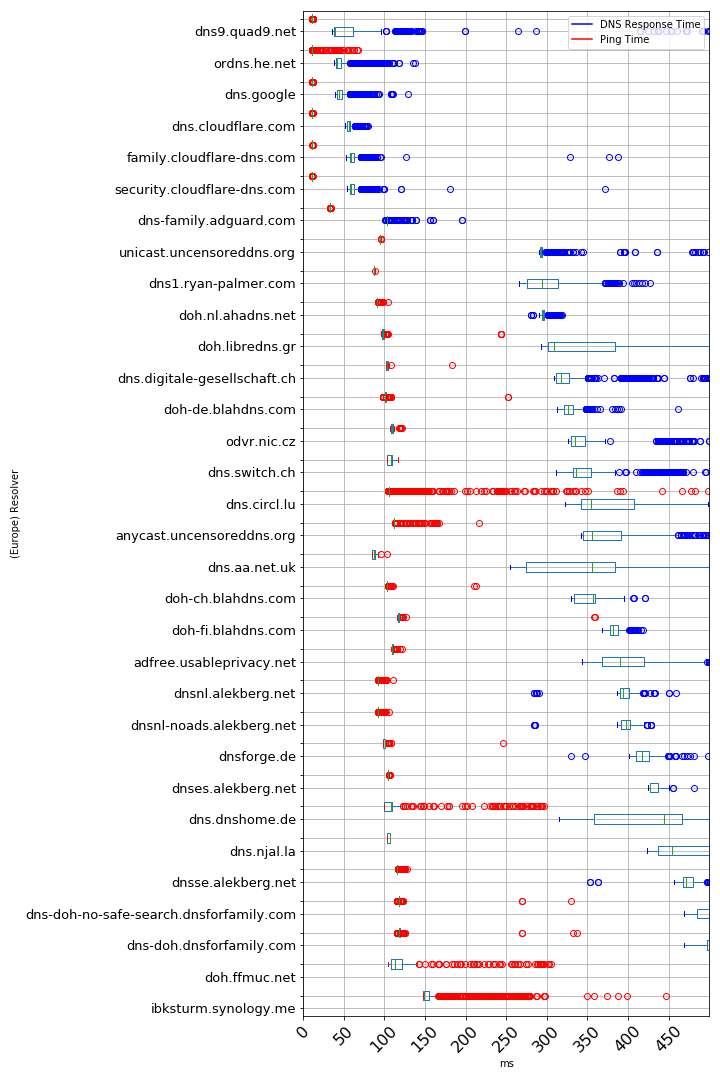
\includegraphics[height=2in]{figures/Ohio_Europe.png}}%
\caption{Resolvers measured from a vantage point in Ohio, USA.}
\end{figure}

\begin{figure}[t!]
\centering
\subfigure[North America.]{%
\label{fig:Seoul_NA}%
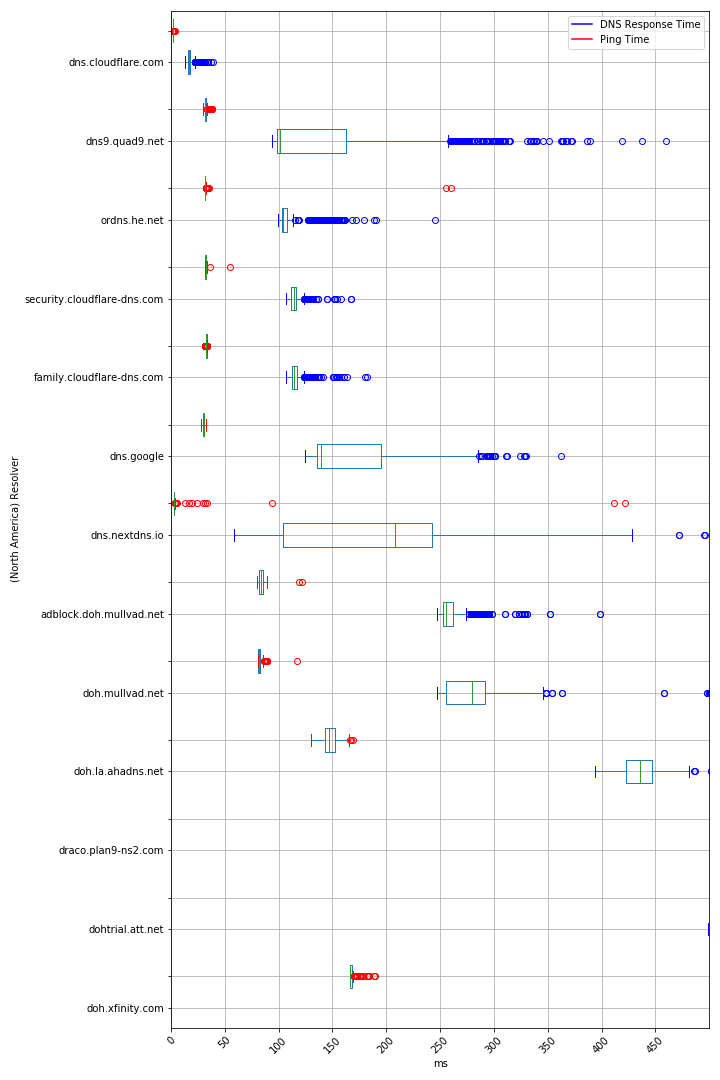
\includegraphics[height=2in]{figures/Seoul_North_America.png}}%
\hspace{8pt}%
\subfigure[Asia.]{%
\label{fig:Seoul_Asia}%
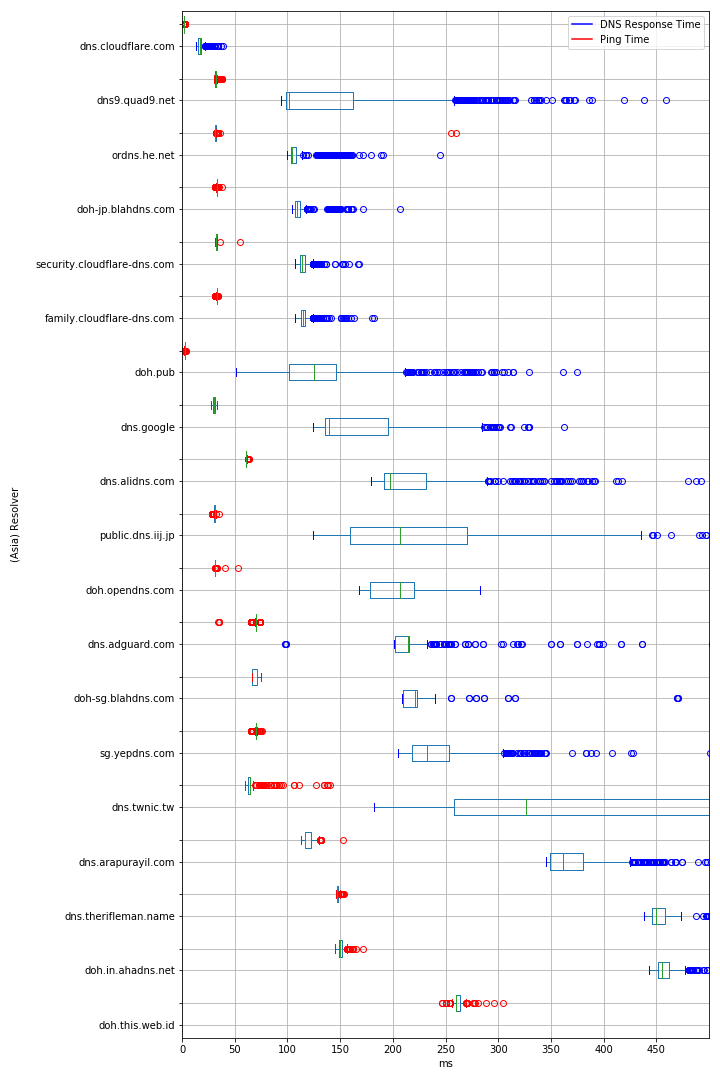
\includegraphics[height=2in]{figures/Seoul_Asia.png}}%
\hspace{8pt}%
\subfigure[Europe.]{%
\label{fig:Seoul_Europe}%
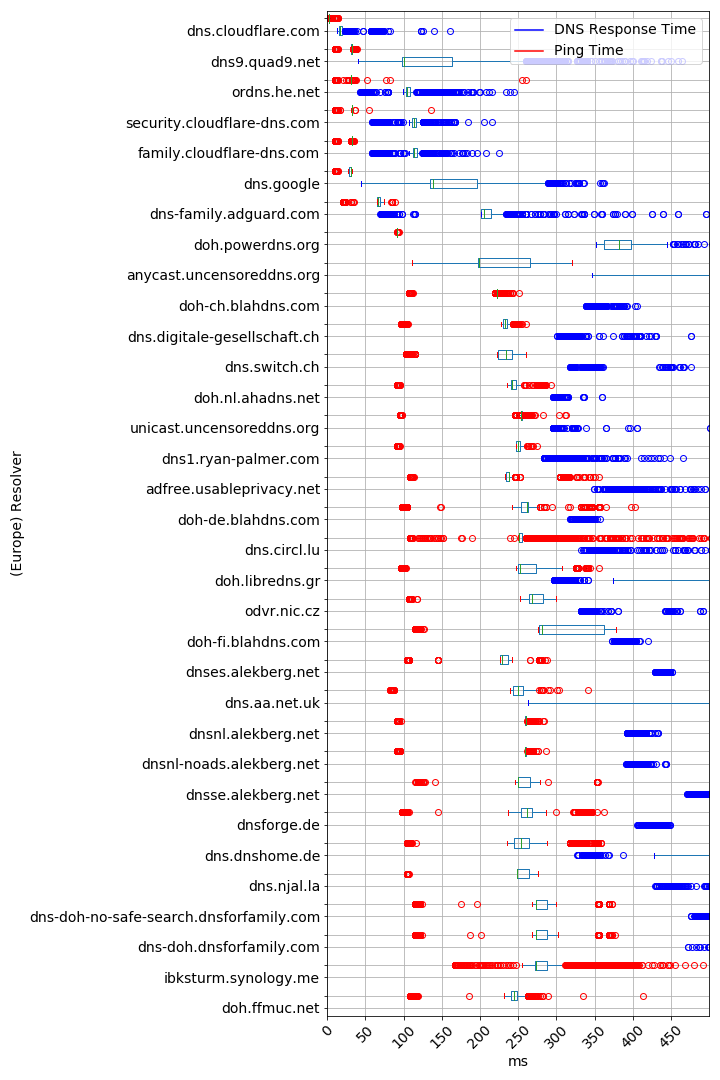
\includegraphics[height=2in]{figures/Seoul_Europe.png}}%
\caption{Resolvers measured from a vantage point in Seoul, South Korea.}
\end{figure}

\begin{figure}[t!]
\centering
\subfigure[North America.]{%
\label{fig:Frankfurt_NA}%
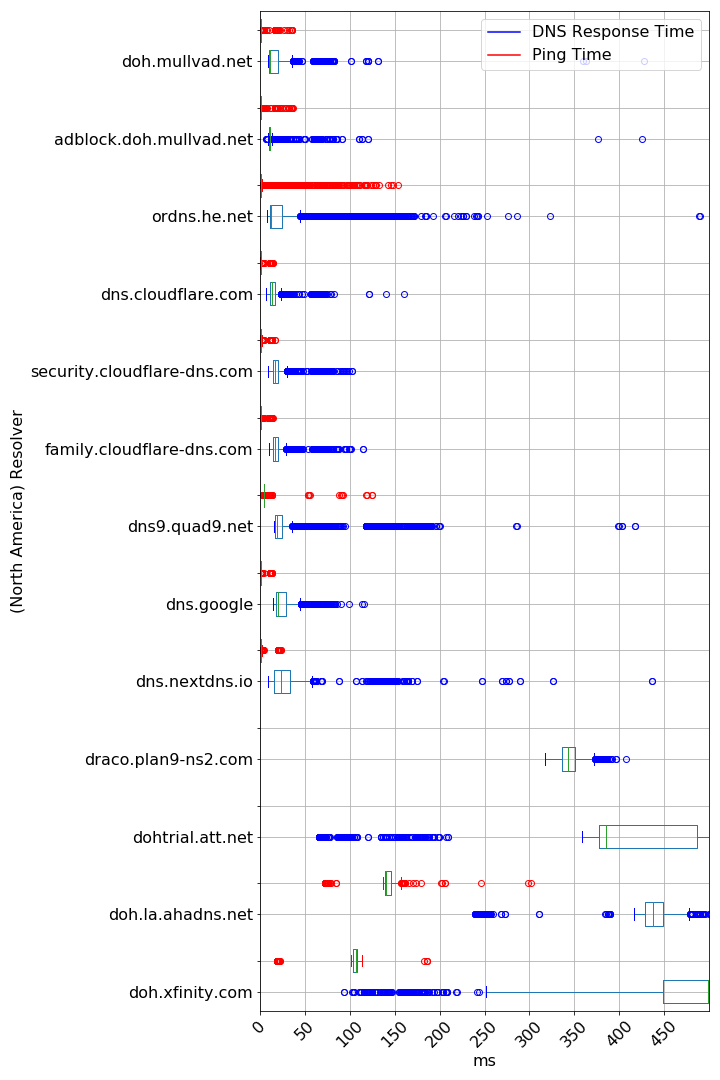
\includegraphics[height=2in]{figures/Frankfurt_North_America.png}}%
\hspace{8pt}%
\subfigure[Asia. ]{%
\label{fig:Frankfurt_Asia}%
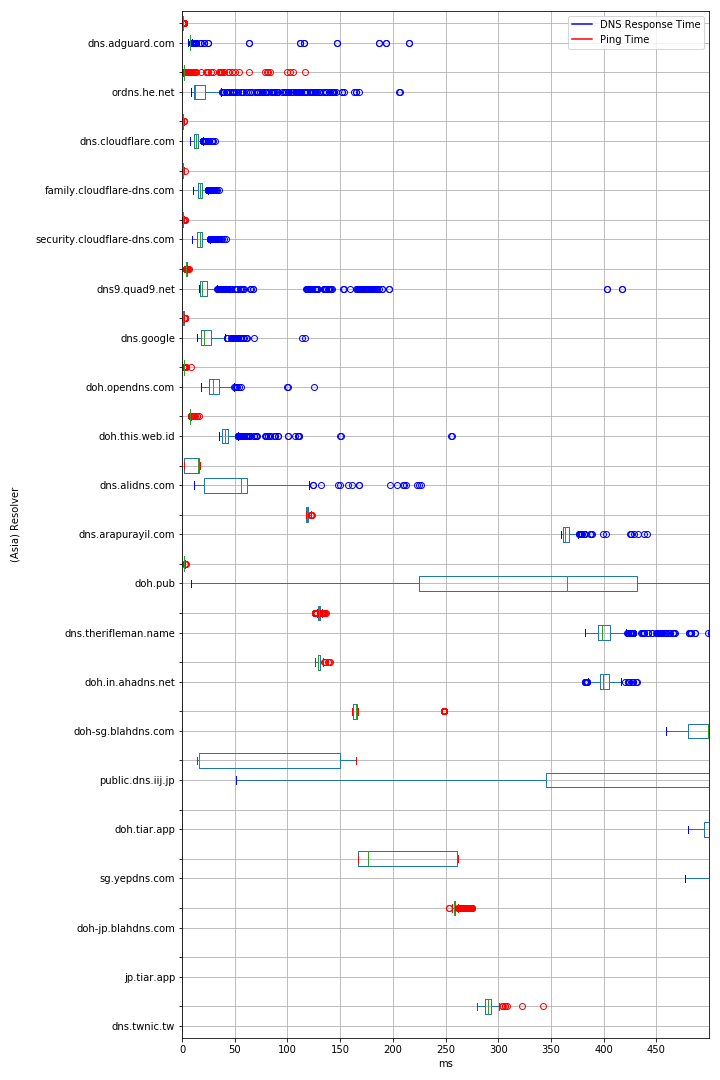
\includegraphics[height=2in]{figures/Frankfurt_Asia.png}}%
\hspace{8pt}%
\subfigure[Europe.]{%
\label{fig:Frankfurt_Europe}%
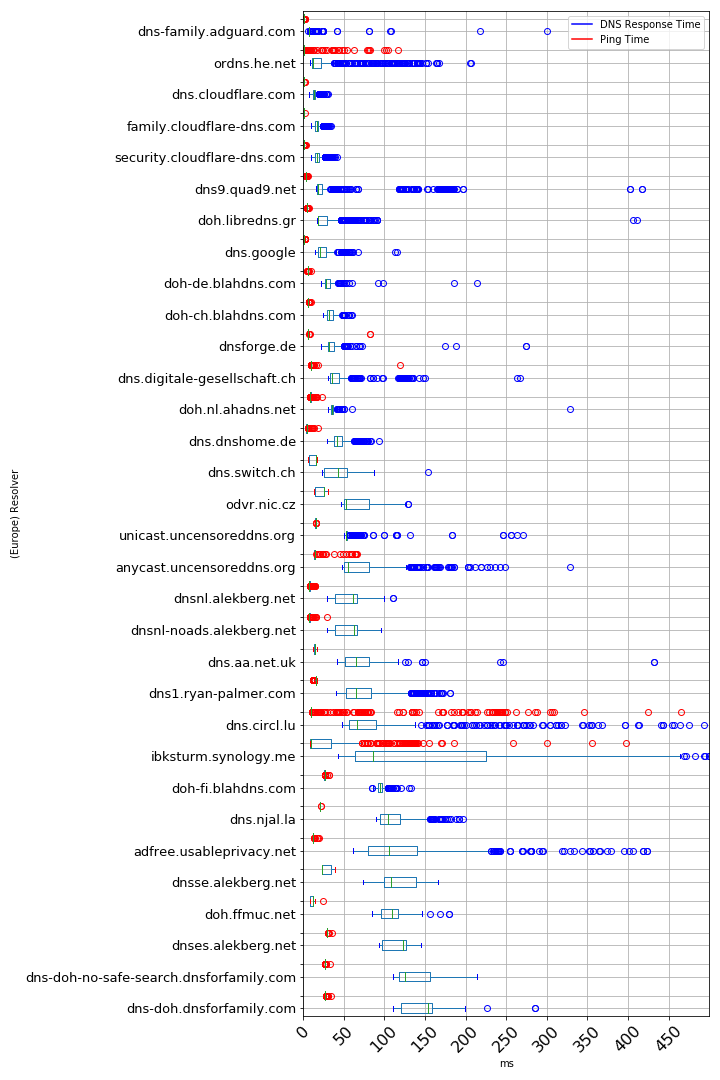
\includegraphics[height=2in]{figures/Frankfurt_Europe.png}}%
\caption{Box-plots of resolvers measured from a vantage point in Frankfurt, Germany}
\end{figure}

\begin{figure}[t!]
\centering
\subfigure[North American resolvers measured from Ohio, USA]{%
\label{fig:Local_Ohio_NA}%
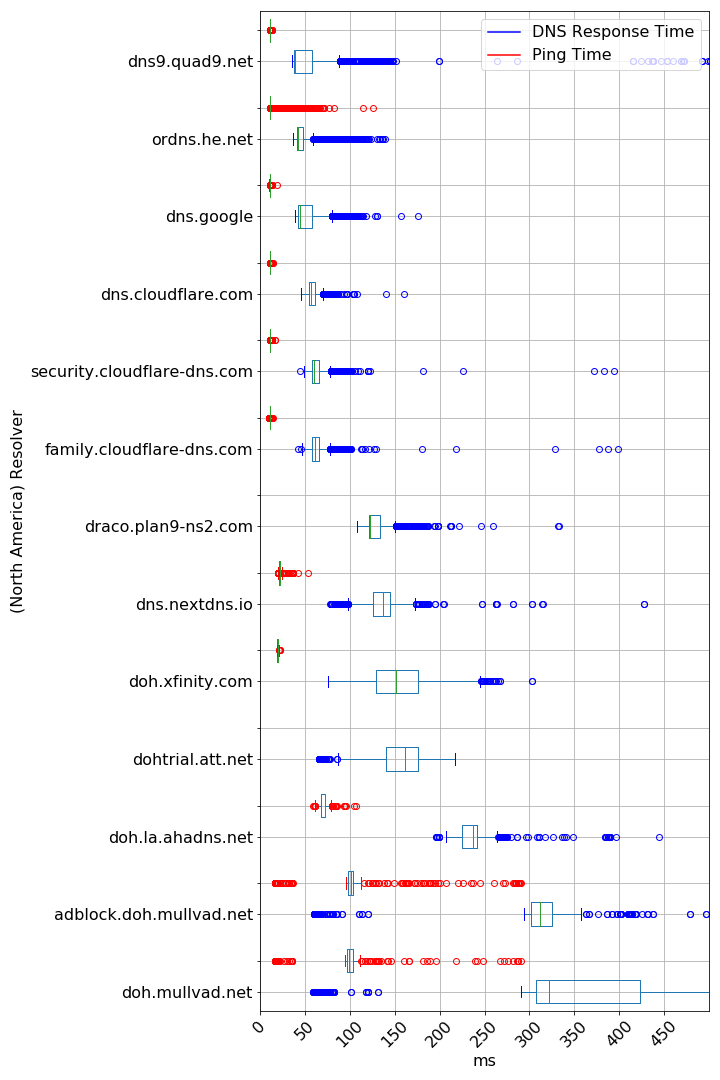
\includegraphics[height=2in]{figures/Ohio_North_America.png}}%
\hspace{8pt}%
\subfigure[Asian resolvers measured from Seoul, South Korea]{%
\label{fig:Local_Seoul_Asia}%
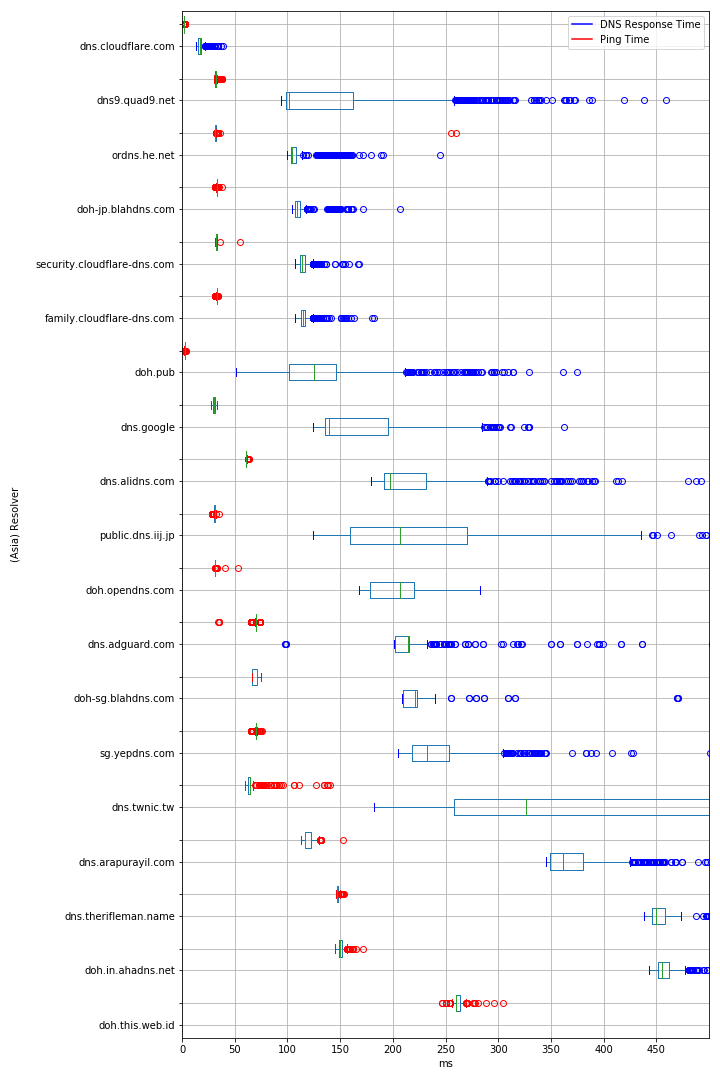
\includegraphics[height=2in]{figures/Seoul_Asia.png}}%
\hspace{8pt}%
\subfigure[European resolvers measured from Frankfurt, Germany]{%
\label{fig:Kocal_Frankfurt_Europe}%
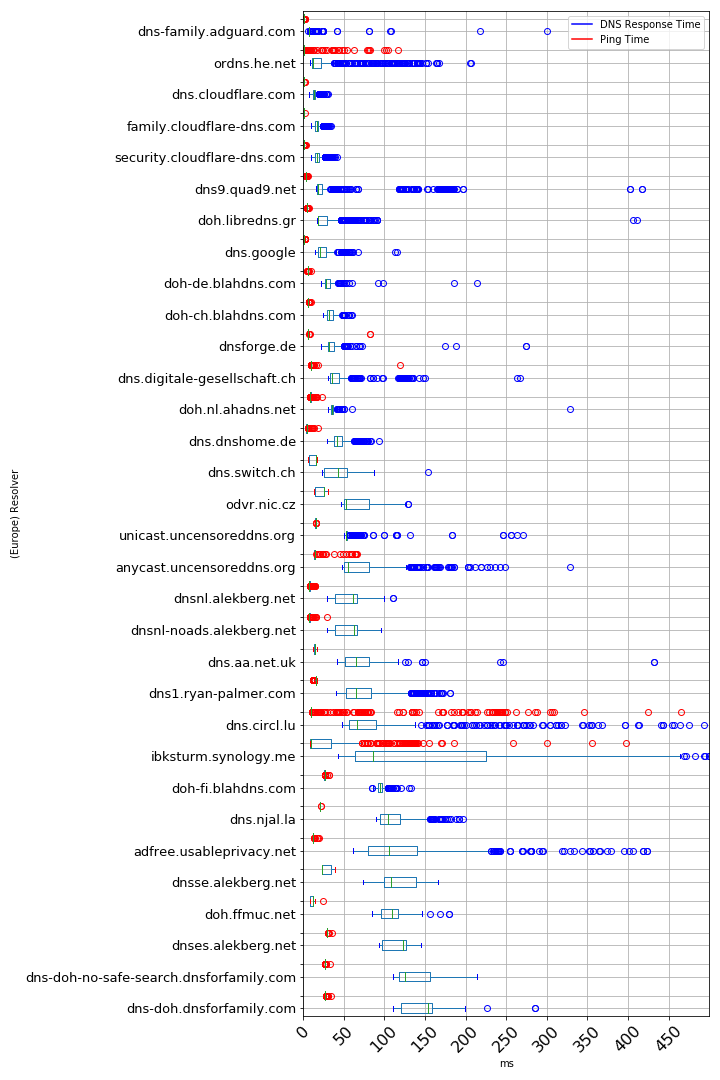
\includegraphics[height=2in]{figures/Frankfurt_Europe.png}}%
\caption{Local-to-local resolvers.}
\end{figure}

\begin{table}[t!]
\centering
\begin{tabular}{ll}
\hline
\textbf{Location} & \textbf{Resolver}                                                                               \\ \hline
North America     & ordns.he.net                                                                                    \\ \hline
Asia              & \begin{tabular}[c]{@{}l@{}}ordns.he.net\\ doh-jp.blahdns.com\end{tabular}                       \\ \hline
Europe            & \begin{tabular}[c]{@{}l@{}}ordns.he.net\\ dns-family.adguard.com\\ doh.libredns.gr\end{tabular} \\ \hline
\end{tabular}
\caption{Non-mainstream resolvers that outperformed mainstream resolvers.}
\label{tab:outperformed_resolvers}
\end{table}

\subsection{How Do Mainstream Resolvers Compare to Non-Mainstream Resolvers?}
We find that, in general, mainstream resolvers outperformed non-mainstream resolvers, with some notable exceptions.
Table~\ref{tab:outperformed_resolvers} compares median response times for major resolvers to non-mainstream resolvers that performed better.
Across all three vantage points, \texttt{dns.quad9.net}, \texttt{dns.google}, and \texttt{dns.cloudflare.com} were among the top five highest performing DoH resolvers.
However, \texttt{ordns.he.net}--a DoH resolver hosted by Hurricane Electric, a global Internet service provider (ISP)--managed to outperform \texttt{dns.google} and \texttt{dns.cloudflare.com} from all three vantage points.
From our vantage point in Frankfurt, we see that \texttt{dns-family.adguard.com} and \texttt{ordns.he.net} are the top two highest performing resolvers.
Finally, from our vantage point in Seoul, we see that \texttt{doh-jp.blahdns.com} outperforms \texttt{dns.google}.

However, most other non-mainstream DoH resolvers performed worse than mainstream resolvers, and they exhibited a wide distribution of median query response times.
For example, from our Ohio vantage point, we observe that outside of the top-five highest performing resolvers, median query response times ranged from \xxx{X} ms to \xxx{X} ms.
From our Seoul vantage point, median response times outside of the top five ranged from \xxx{X} ms to \xxx{X} ms.
We observe more consistent performance overall from our Frankfurt vantage point, but we still see median query response times outside the top five range from \xxx{X} ms to \xxx{X} ms.

\subsection{Does Network Distance Correlate to High Response Times from Non-Mainstream Resolvers?}
\begin{table}[ht]
\centering
\begin{tabular}{lll}
\toprule
\textbf{Resolver} & \textbf{Vantage Point} & \\
                  & \textbf{Seoul}         & \textbf{Frankfurt} \\
\midrule
dns.twnic.tw                                & 326.19                                           & 32374.03                            \\
doh-jp.blahdns.com                          & 109.41                                           & 754.26                              \\
sg.yepdns.com                               & 232.69                                           & 540.19                              \\
public.dns.iij.jp                           & 206.37                                           & 506.05                              \\
doh-sg.blahdns                              & 221.41                                           & 498.76                              \\
\bottomrule
\end{tabular}
\caption{Median DNS response times for non-conventional resolvers located in Asia.}
\label{tab:UnconvAsia}
\end{table}

\begin{table}[ht]
\centering
\begin{tabular}{lll}
\toprule
\textbf{Resolver} & \textbf{Vantage Point} & \\
                  & \textbf{Frankfurt}     & \textbf{Seoul} \\
\midrule
doh.ffmuc.net                               & 109.15                                           & 1307.21                         \\
ibksturm.synology.me                        & 85.77                                            & 1227.35                         \\
dns-doh-no-safe-search.dnsforfamily         & 125.74                                           & 1150.63                         \\
dnsforge.de                                 & 32.17                                            & 1029.92                         \\
dns-doh.dnsforfamily                        & 153.74                                           & 1153.29                         \\
\bottomrule
\end{tabular}
\caption{Median DNS response times for non-conventional resolvers located in Europe.}
\label{tab:UnconvEur}
\end{table}

In general, we find that network distance correlates to higher median response times.
\Fref{tab:UnconvAsia} shows that non-conventional resolvers located in Asia perform better from the Seoul vantage point than the Frankfurt vantage point. 
Similarly, \Fref{tab:UnconvEur} demonstrates that the response times of European non-conventional resolvers measured from Frankfurt are much lower than the response times of those same resolvers measured from Seoul.

However, certain resolvers performed significantly worse than their network distance might imply.
For example, although the average latency we observed to \texttt{doh.in.ahadns.net} from our Seoul vantage point was \xxx{X} ms, the median query response time was \xxx{X} ms.
Similarly, from our Ohio vantage point, we observed an average latency to \texttt{doh.xfinity.com} of \texttt{X} ms, despite a median query response time of \xxx{X} ms.
We believe this could be attributed these non-mainstream resolvers having especially smaller caches than mainstream resolvers.
These resolvers may perform better in the future as more clients use them and populate their caches.
\AH{Review this previous hypothesis later}
We note that certain resolvers did not respond to our ICMP ping messages (\Fref{tab:unresponsive}).

\subsection{How Many Non-Mainstream Resolvers Are Responsive?}
\begin{table}[ht]
\centering
\begin{tabular}{lllll}
\hline
\textbf{Location} & \textbf{Resolver} & \textbf{Responsive?} & & \\
    & & \textbf{Ohio} & \textbf{Seoul} & \textbf{Frankfurt} \\
\midrule
North America     & \begin{tabular}[c]{@{}l@{}}dnscrypt.ca-1-doh\\ dnscrypt.ca-2-doh\\ doh-cleanbrowsing\\ doh.post-factum.tk\end{tabular} & \begin{tabular}[c]{@{}l@{}}No\\ No\\ No\\ No\end{tabular} & \begin{tabular}[c]{@{}l@{}}No\\ No\\ No\\ No\end{tabular} & \begin{tabular}[c]{@{}l@{}}No\\ No\\ No\\ No\end{tabular}    \\ \midrule
Asia              & \begin{tabular}[c]{@{}l@{}}doh.tiarap.org\\ jp.tiarap.org\\ doh.linuxsec\end{tabular} & \begin{tabular}[c]{@{}l@{}}No\\ No\\ No\end{tabular}      & \begin{tabular}[c]{@{}l@{}}No\\ No\\ No\end{tabular}      & \begin{tabular}[c]{@{}l@{}}Yes\\ Yes\\ No\end{tabular}            \\ \midrule
Europe            & \begin{tabular}[c]{@{}l@{}}doh.bortzmeyer\\ doh.appliedprivacy\\ doh.chewbacca.meganerd.nl\\ doh.powerdns\end{tabular} & \begin{tabular}[c]{@{}l@{}}No\\ No\\ No\\ No\end{tabular} & \begin{tabular}[c]{@{}l@{}}No\\ No\\ No\\ No\end{tabular} & \begin{tabular}[c]{@{}l@{}}No\\ No\\ No\\ No\end{tabular} \\ \bottomrule
\end{tabular}
\caption{Resolvers that failed to respond from each vantage point.}
\label{tab:unresponsive}
\end{table}
\Fref{tab:unresponsive} list the DoH resolvers that we failed to receive a response from.
\Fref{tab:errors} also breaks down the most common errors we received from attempting to communicate with unresponsive resolvers.
We find that most resolvers we measured were responsive, albeit some reported relatively high median query response times.
For the resolvers that we did not receive responses from, the most common errors related to a failure to establish a TCP connection or a TLS session.
\AH{Review this previous sentence later with the full data}
In other words, when we didn't receive a response, it wasn't necessarily because the response itself was dropped on-path or our software reported a timeout, but rather that the server was likely no longer operational in the first place.

\label{lastpage}\section{Conclusion}\label{sec:conclusion}

In this work, we investigated the DNS response of times of a set of global DoH
resolvers from different vantage points.  We find that although most
lesser-known resolvers have higher response times than well-known resolvers, a
select group of lesser-known resolvers had close response times, or even lower
response times, to well-known resolvers.  Additionally, we find a wide
distribution of response times between resolvers despite their close proximity
to one another.  Many of the non-mainstream resolvers are restricted based off
of their location.  

Our results suggest that while clients may generally expect the best DoH query response times with current major resolvers, they may also use certain less-popular resolvers within their geographic region.
They also suggest that any resolver that is not majorly deployed is not useful if it is outside of one's region.
Of the \xxx{X} non-mainstream resolvers we measured, \xxx{X} performed within 10ms in median query response times for Clouflare, \xxx{X} for Google, and \xxx{X} for Quad9.

Furthermore, \xxx{X} of these non-mainstream resolvers were among the top five highest performing resolvers for a given vantage point.
Several of these resolvers were hosted by ISPs.
Thus, as more ISPs deploy DoH, we expect that clients will have even greater choice among which resolvers they use.

Previous work suggests DoH response times may not greatly matter for certain applications, such as web browsers.
Hounsel et al. found that while DoH response times were generally higher than traditional DNS, page load times were comparable~\cite{hounsel2020comparing}.
These measurements were performed with major DoH resolvers--namely Cloudflare, Google, and Quad9--but the results should generalize.
DoH connections based on HTTP/2 and above may utilize asynchronous queries, enabling the browser to send multiple DoH queries.
In short, if applications enable DoH queires to be asynchronously issued, and TCP/TLS sessions are re-used with long timeouts, then higher DNS response times from non-mainstream resolvers witin a client's geographic region may not matter.
Future work could measure page load times alongside DNS response times.  This
would provide greater insight into how user experience is directly impacted by
resolver performance.  Measurements of DoT resolvers could also be collected
to compare with DoH resolvers and understand if both are impacted by network
distance in the same way. 


\pagebreak
\bibliographystyle{splncs04}
\bibliography{paper}

\appendix
\section{Appendix}

\subsection{Additional Figures}
\begin{figure}[h!]
\hspace*{-1in}
\begin{minipage}{1.35\textwidth}
\centering
\subfigure[North America (Local).]{%
\label{fig:Ohio_NA_Appendix}%
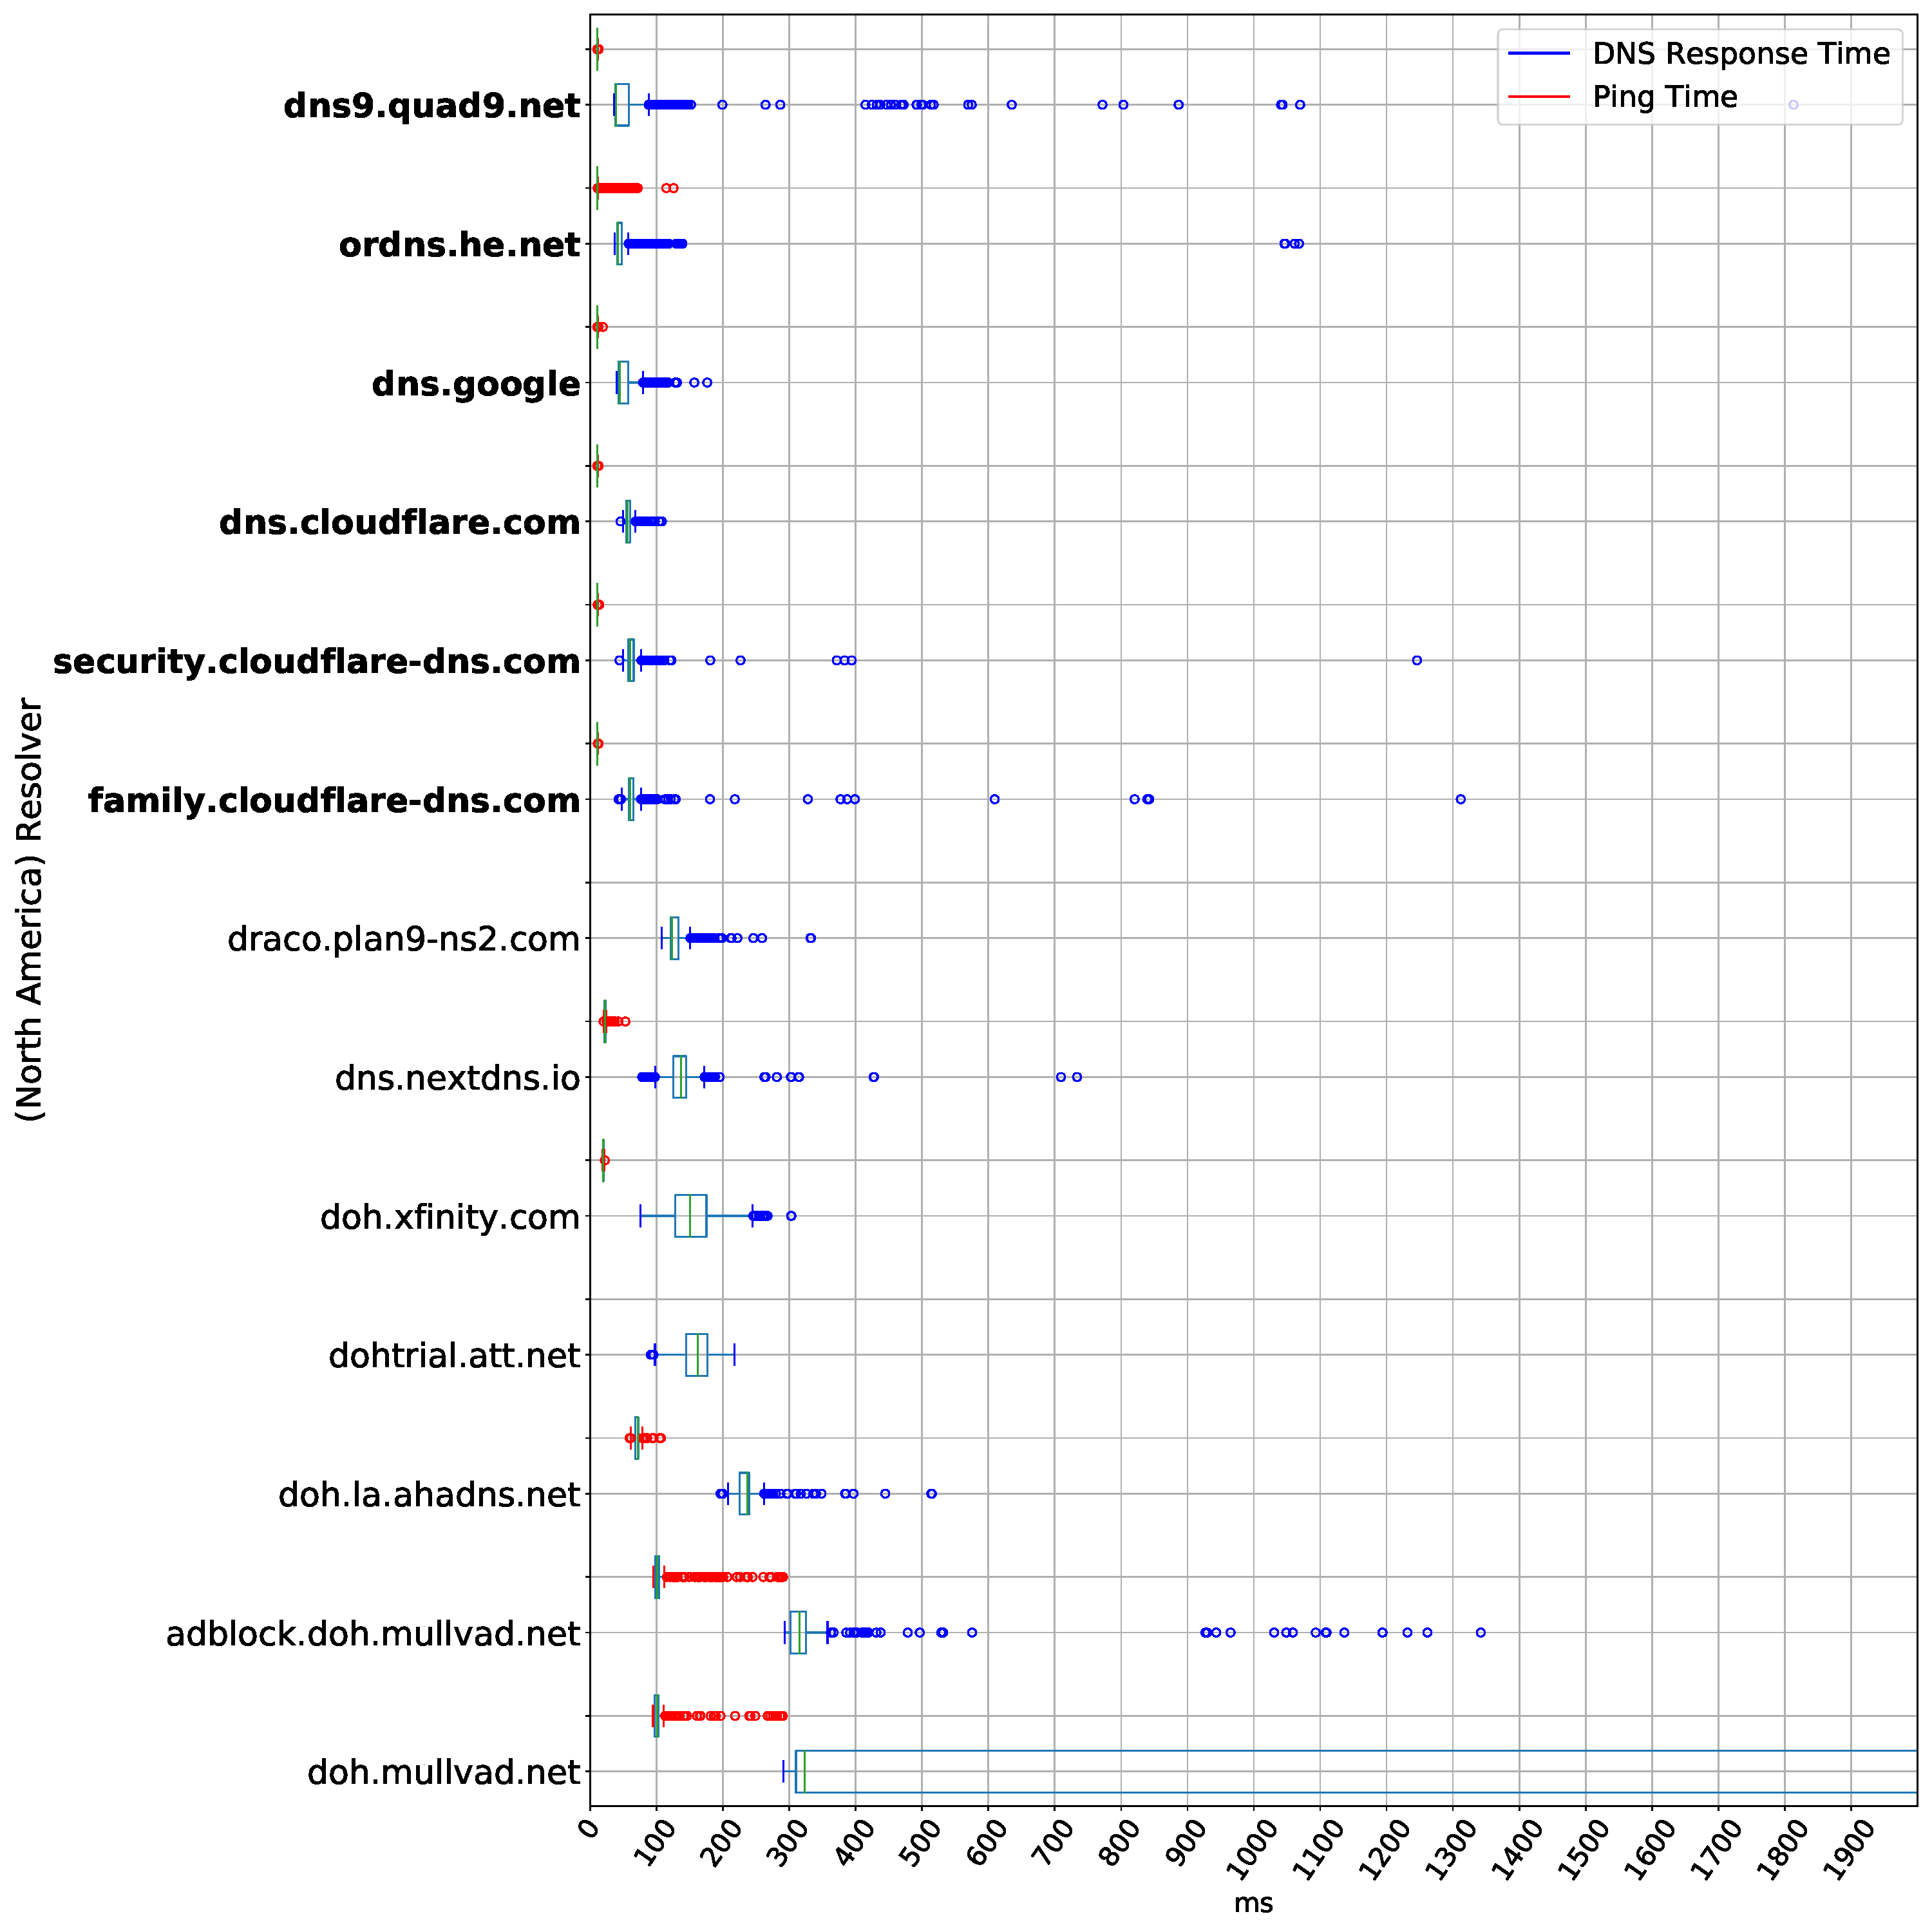
\includegraphics[width=0.32\linewidth]{figures/Ohio_North_America_Full.pdf}}%
\hfill%
    \subfigure[Asia (Local).]{%
\label{fig:Seoul_Asia_Appendix}%
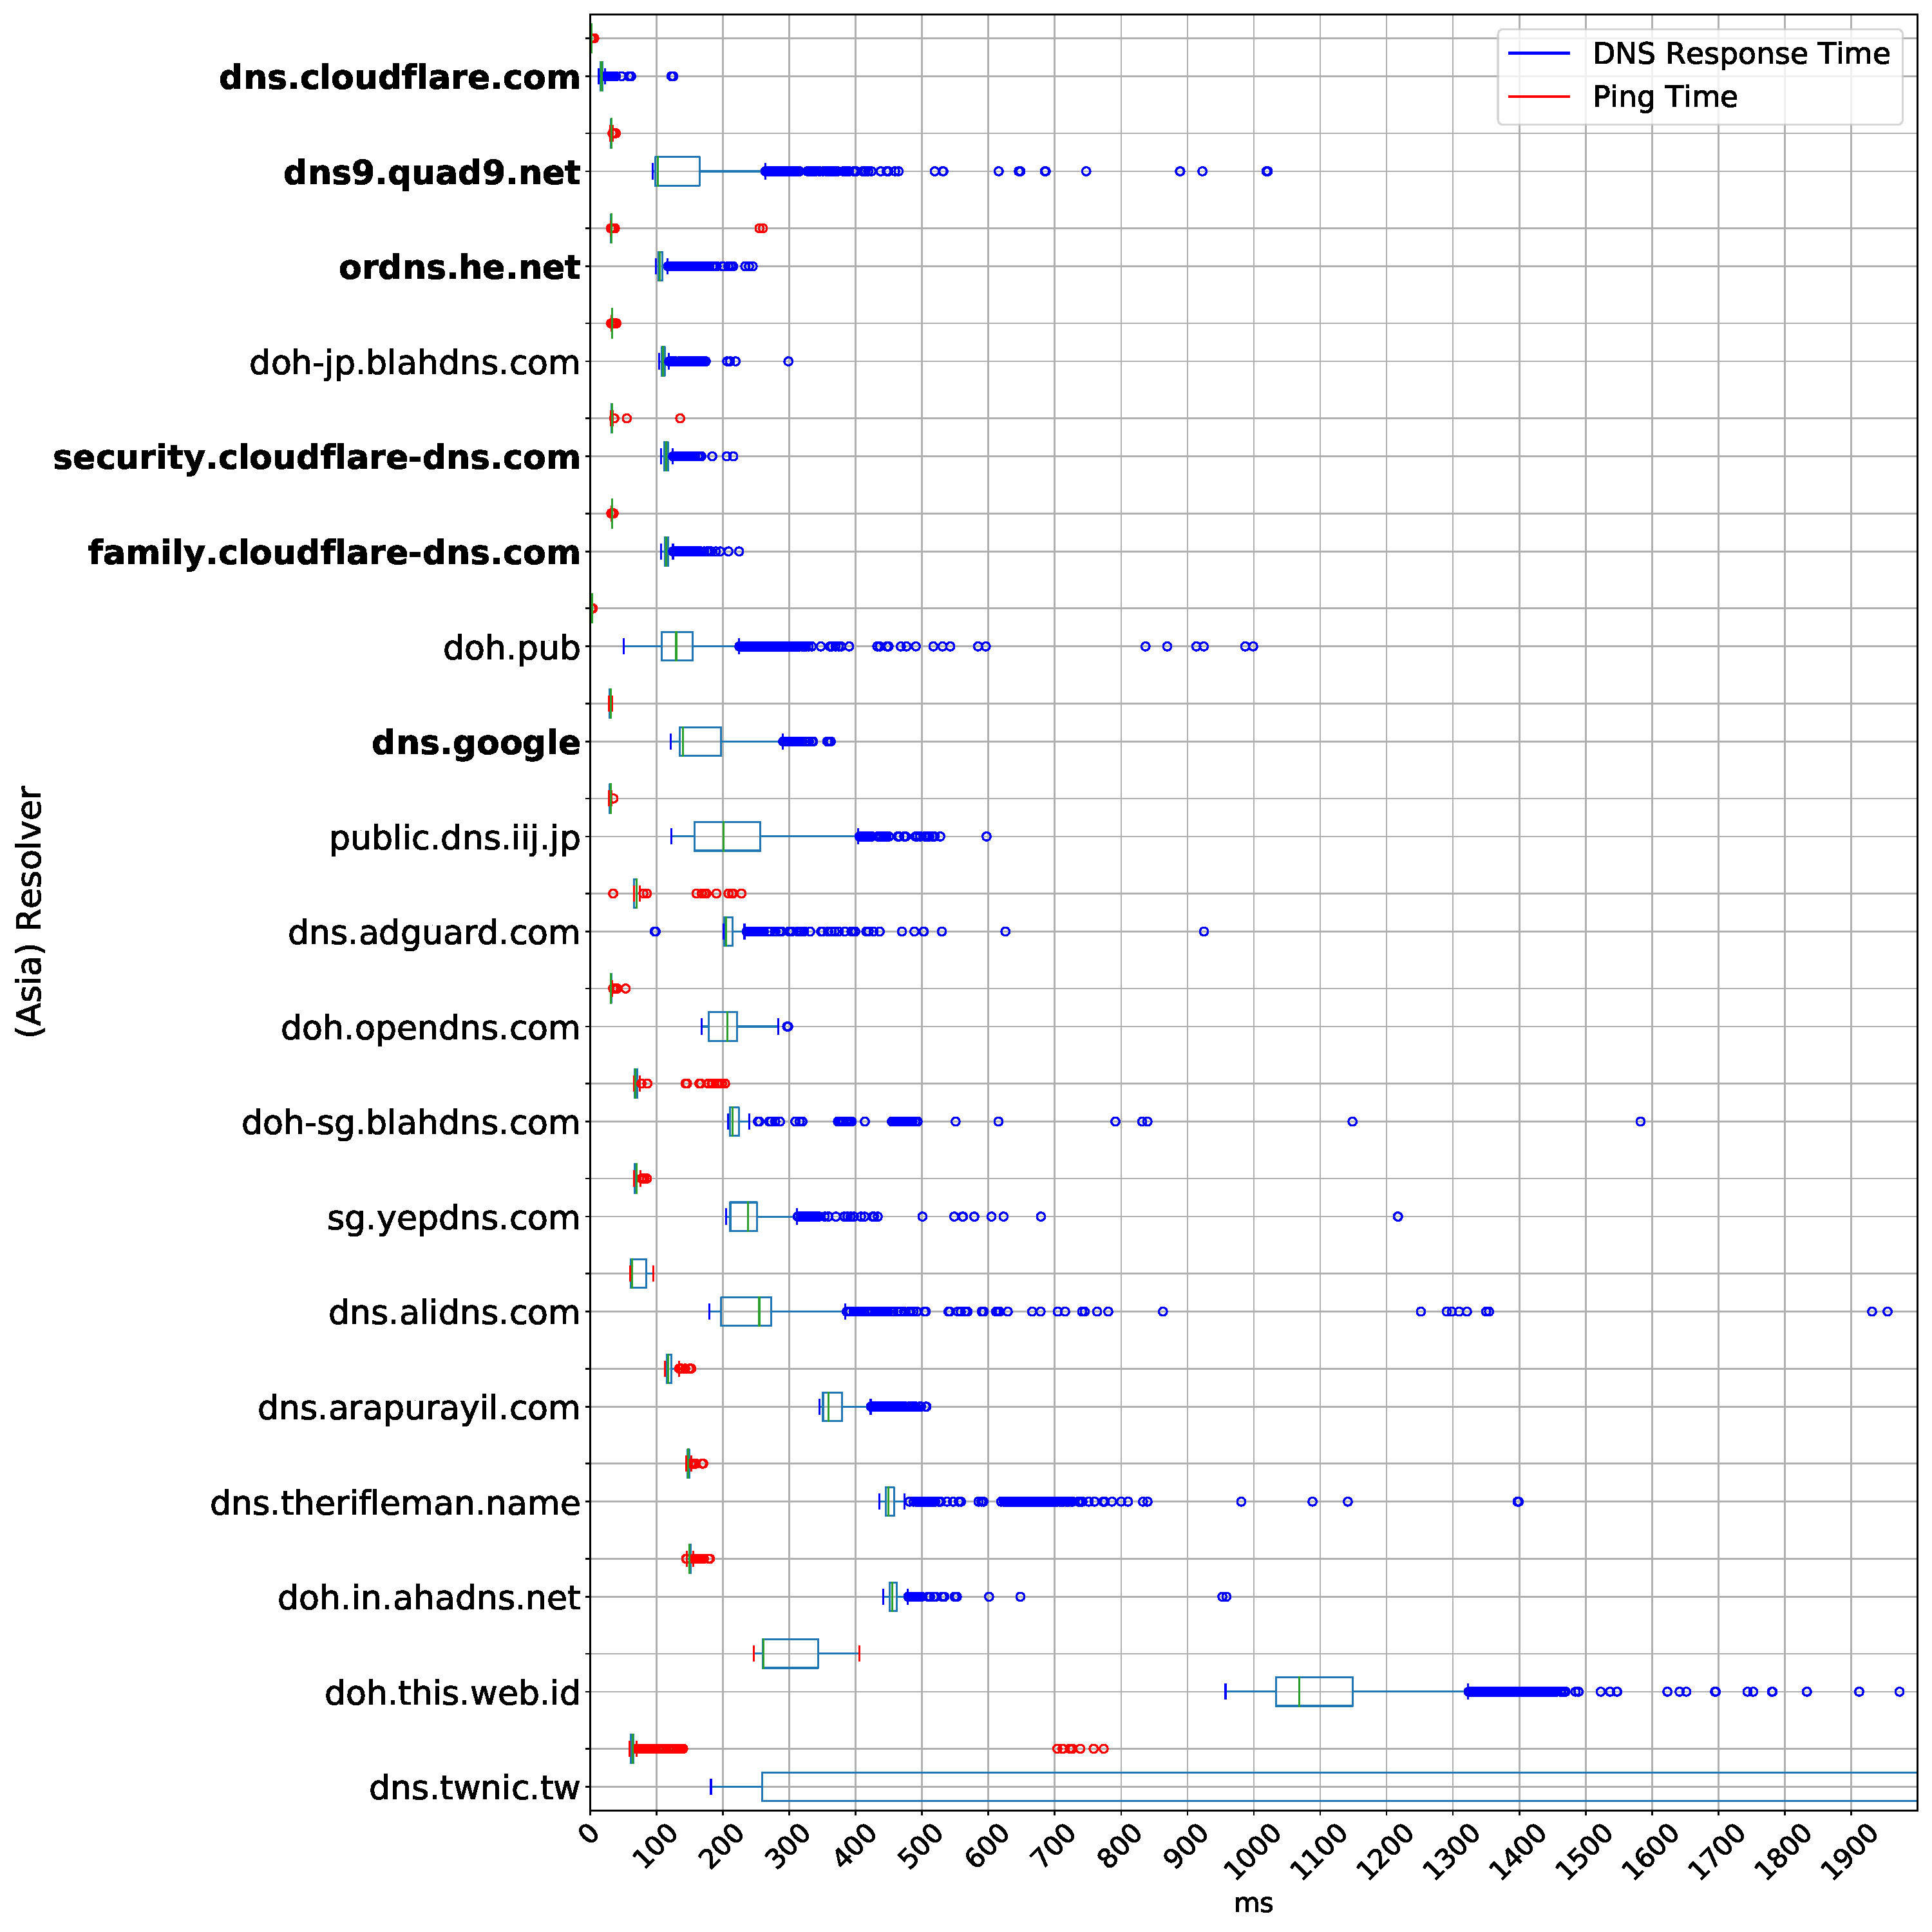
\includegraphics[width=0.32\linewidth]{figures/Seoul_Asia_Full.pdf}}%
\hfill%
\subfigure[Europe (Local).]{%
\label{fig:Frankfurt_Europe_Appendix}%
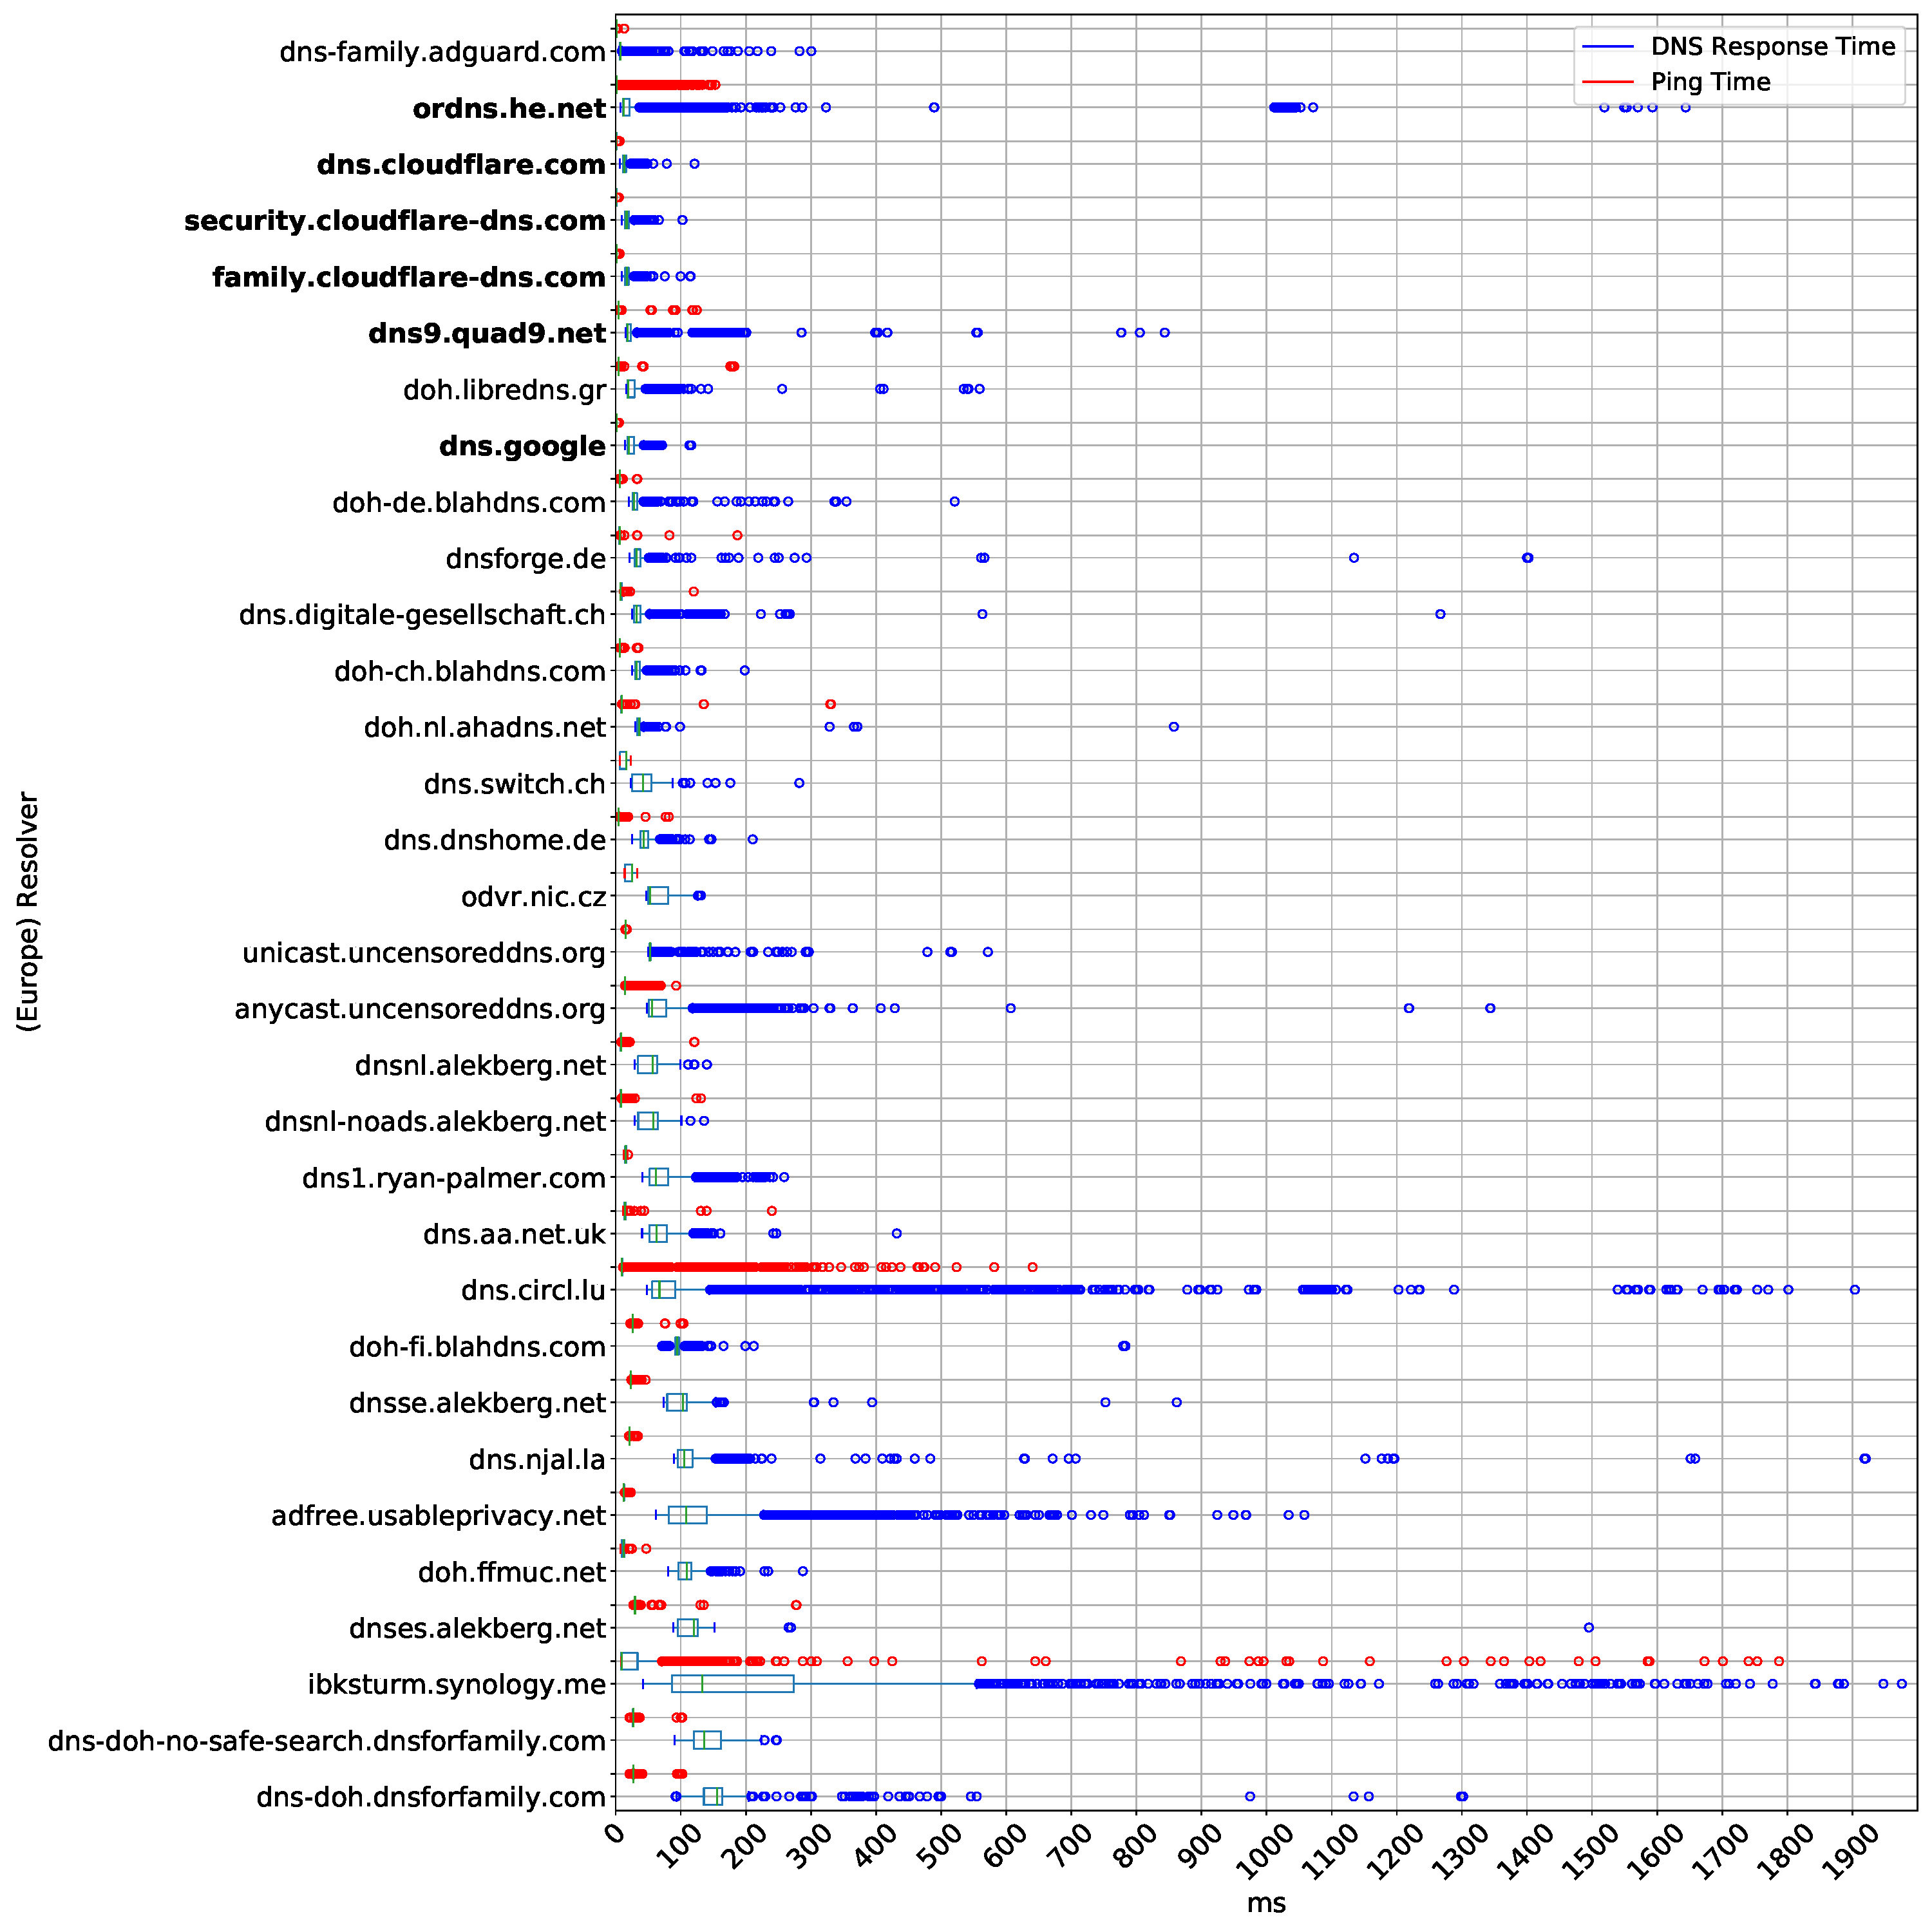
\includegraphics[width=0.32\linewidth]{figures/Frankfurt_Europe_Full.pdf}}%
\caption{Resolvers measured from local vantage points. These plots do not 
    cut off response times at 500 ms.}
\end{minipage}
\end{figure}

\subsection{Resolvers}\label{sec:resolvers}
\begin{itemize}
\item https://dns.google/dns-query
\item https://dns.aa.net.uk/dns-query
\item https://adfree.usableprivacy.net/dns-query
\item https://dns.adguard.com/dns-query
\item https://dns-family.adguard.com/dns-query
\item https://doh.in.ahadns.net/dns-query
\item https://doh.la.ahadns.net/dns-query
\item https://doh.nl.ahadns.net/dns-query
\item https://dns.alidns.com/dns-query
\item https://dnsnl-noads.alekberg.net/dns-query
\item https://dnsnl.alekberg.net/dns-query
\item https://dns.arapurayil.com/dns-query
\item https://dohtrial.att.net/dns-query
\item https://dnses.alekberg.net/dns-query
\item https://doh.bortzmeyer.fr/dns-query
\item https://dns.circl.lu/dns-query
\item https://doh.opendns.com/dns-query
\item https://dns.cloudflare.com/dns-query
\item https://family.cloudflare-dns.com/dns-query
\item https://security.cloudflare-dns.com/dns-query
\item https://odvr.nic.cz/dns-query
\item https://dns.digitale-gesellschaft.ch/dns-query
\item https://dns.digitale-gesellschaft.ch/dns-query
\item https://dns1.ryan-palmer.com/dns-query
\item https://doh.sb/dns-query
\item https://dns.therifleman.name/dns-query
\item https://dns1.dnscrypt.ca/dns-query
\item https://dns2.dnscrypt.ca/dns-query
\item https://dns-doh.dnsforfamily.com/dns-query
\item https://dns-doh-no-safe-search.dnsforfamily.com/dns-query
\item https://dnsforge.de/dns-query
\item https://dns.dnshome.de/dns-query
\item https://doh.pub/dns-query
\item https://doh-ch.blahdns.com/dns-query
\item https://doh.cleanbrowsing.org/dns-query
\item https://doh.cleanbrowsing.org/dns-query
\item https://doh.cleanbrowsing.org/dns-query
\item https://doh.crypto.sx/dns-query
\item https://doh-de.blahdns.com/dns-query
\item https://doh-fi.blahdns.com/dns-query
\item https://ibksturm.synology.me/dns-query
\item https://doh-jp.blahdns.com/dns-query
\item https://doh-sg.blahdns.com/dns-query
\item https://doh.appliedprivacy.net/dns-query
\item https://doh.ffmuc.net/dns-query
\item https://doh.tiarap.org/dns-query
\item https://ordns.he.net/dns-query
\item https://doh.tiar.app/dns-query
\item https://public.dns.iij.jp/dns-query
\item https://doh.this.web.id/dns-query
\item https://jp.tiar.app/dns-query
\item https://jp.tiarap.org/dns-query
\item https://doh.libredns.gr/dns-query
\item https://doh.libredns.gr/dns-query
\item https://doh.linuxsec.org/dns-query
\item https://doh.linuxsec.org/dns-query
\item https://adblock.doh.mullvad.net/dns-query
\item https://doh.chewbacca.meganerd.nl/dns-query
\item https://doh.mullvad.net/dns-query
\item https://dns.nextdns.io/dns-query
\item https://dns.njal.la/dns-query
\item https://doh.post-factum.tk/dns-query
\item https://draco.plan9-ns2.com/dns-query
\item https://doh.powerdns.org/dns-query
\item https://doh.seby.io/dns-query
\item https://doh-2.seby.io/dns-query
\item https://dns.twnic.tw/dns-query
\item https://dns9.quad9.net/dns-query
\item https://dns9.quad9.net/dns-query
\item https://dnsse.alekberg.net/dns-query
\item https://dns.switch.ch/dns-query
\item https://dns.t53.de/dns-query
\item https://unicast.uncensoreddns.org/dns-query
\item https://anycast.uncensoreddns.org/dns-query
\item https://sg.yepdns.com/dns-query
\item https://doh.xfinity.com/dns-query
\end{itemize}


\end{sloppypar}
\end{document}

%%%%%%%%%%%%%%%%%%%%  END OF DOCUMENT  %%%%%%%%%%%%%%%%%%%%
